\documentclass[10pt,svgnames,usenames,table]{beamer} %,handout si version papier
\NeedsTeXFormat{LaTeX2e}

\usetheme[compress]{Singapore} % theme

\usepackage[frenchb]{babel}
\usepackage[T1]{fontenc}
\usepackage[utf8x]{inputenc}
\usepackage{lmodern}
\usepackage{amsmath,amsthm,amssymb}        % un packages mathématiques
\usepackage{xcolor}         % pour définir plus de couleurs
\usepackage{graphicx}       % pour insérer des figures
\usepackage{lmodern}
\usepackage{url}
	\urlstyle{sf}
\usepackage{lastpage}
\usepackage{endnotes}

\usepackage{listings}
\usepackage{listingsutf8}

\usepackage{siunitx}
\usepackage{circuitikz}
\usepackage{chemfig}
\usepackage[version=3]{mhchem}

\usepackage[french]{varioref}
\usepackage{wrapfig}
\usepackage{pdfpages}
\usepackage{verbatim}
\usepackage{graphicx}

%\usepackage[svgnames]{color}
%\definecolor{webdarkblue}{rgb}{0,0,0.4}
%\definecolor{webgreen}{rgb}{0,0.3,0}
%\definecolor{webblue}{rgb}{0,0,0.8}

\setbeamercolor{section in head/foot}{use=structure,bg=structure.fg!25!bg} % "Amélioration du jeu de couleur"
%\useoutertheme[subsection=true]{smoothbars} % Pour avoir un rappel de la subsection
\setbeamerfont{frametitle}{series=\bfseries}
\setbeamertemplate{frametitle}[default][center] % Titre centré et bien placé.


% "Fioriture de style" : qd <x-> dans les item, les autres en gris clair
\beamertemplatetransparentcovered


% Comportement des itemize
\setbeamertemplate{itemize item}[ball]
\setbeamertemplate{itemize subitem}[triangle]
\setbeamertemplate{itemize subsubitem}[circle]

%\renewcommand\sfdefault{cmss} % Polices

% Les block arrondis et ombrés dans la couleur que je veux
\setbeamertemplate{blocks}[rounded][shadow=true]
\definecolor{normalBlockColor}{RGB}{255,255,255}
\definecolor{normalTitleBlockColor}{RGB}{0,0,102}
\definecolor{normalBlockTextColor}{RGB}{0,0,0}
\definecolor{normalBlockTitleTextColor}{RGB}{255,255,255}
\definecolor{exampleBlockColor}{RGB}{202,251,197}
\definecolor{exampleTitleBlockColor}{RGB}{166,241,158}
\definecolor{exampleBlockTextColor}{RGB}{0,0,0}
\definecolor{exampleBlockTitleTextColor}{RGB}{0,120,0}
\definecolor{alertBlockColor}{RGB}{248,218,218}
\definecolor{alertTitleBlockColor}{RGB}{244,108,108}
\definecolor{alertBlockTextColor}{RGB}{0,0,0}
\definecolor{alertBlockTitleTextColor}{RGB}{120,0,0}
\setbeamercolor*{block title}{fg=normalBlockTitleTextColor,bg=normalTitleBlockColor}
\setbeamercolor*{block body}{fg=normalBlockTextColor,bg=normalBlockColor}
\setbeamercolor*{block title alerted}{fg=alertBlockTitleTextColor,bg=alertTitleBlockColor}
\setbeamercolor*{block body alerted}{fg=alertBlockTextColor,bg=alertBlockColor}
\setbeamercolor*{block title example}{fg=exampleBlockTitleTextColor,bg=exampleTitleBlockColor}
\setbeamercolor*{block body example}{fg=exampleBlockTextColor,bg=exampleBlockColor}
\setbeamerfont{block title}{size={}}



%------------ fin style beamer -------------------

% Faire apparaître un sommaire avant chaque section
% \AtBeginSection[]{
%   \begin{frame}
%   \frametitle{Plan}
%   \medskip
%   %%% affiche en début de chaque section, les noms de sections et
%   %%% noms de sous-sections de la section en cours.
%   \small \tableofcontents[currentsection, hideothersubsections]
%   \end{frame}
% }


% Pour personnaliser la barre de navigation du dessous
\setbeamertemplate{navigation symbols}{
	%\insertslidenavigationsymbol
	%\insertframenavigationsymbol
	%\insertsubsectionnavigationsymbol
	\quad\textbf{\insertframenumber/\inserttotalframenumber} % Numéro de page
	%\insertsectionnavigationsymbol
	%\insertdocnavigationsymbol
	%\insertbackfindforwardnavigationsymbol
}
% Supprimer les icones de navigation (pour les transparents)
%\setbeamertemplate{navigation symbols}{}

% Mettre les icones de navigation en mode vertical (pour projection)
% \setbeamertemplate{navigation symbols}[vertical]

\newenvironment{itemize2}%
	{ \begin{list}%
		{$\bullet$}%
		{\setlength{\labelwidth}{30pt}%
		 \setlength{\leftmargin}{35pt}%
		 \setlength{\itemsep}{\parsep}}}%
	{ \end{list} }

\def\siecle#1{\textsc{\romannumeral #1}\textsuperscript{e}~siècle} % => le \siecle{19}

\definecolor{codeBlue}{rgb}{0,0,1}
\definecolor{webred}{rgb}{0.5,0,0}
\definecolor{codeGreen}{rgb}{0,0.5,0}
\definecolor{codeGrey}{rgb}{0.6,0.6,0.6}
\definecolor{webdarkblue}{rgb}{0,0,0.4}
\definecolor{webgreen}{rgb}{0,0.3,0}
\definecolor{webblue}{rgb}{0,0,0.8}
\definecolor{orange}{rgb}{0.7,0.1,0.1}
\lstset{
      language=C++,
      flexiblecolumns=true,
      numbers=left,
      stepnumber=1,
      numberstyle=\ttfamily\tiny,
      keywordstyle=\ttfamily\textcolor{blue},
      stringstyle=\ttfamily\textcolor{red},
      commentstyle=\ttfamily\textcolor{codeGreen},
      breaklines=true,
      extendedchars=true,
      basicstyle=\ttfamily\scriptsize,
      showstringspaces=false,
      morekeywords={usepackage,documentclass,begin,textbf,textit,texttt,ref,includegraphics,caption,label,setlength,mathbb,notag,frac,num,si,ang,SI,textwidth,percent,meter,ohm,joule,second,more,section,subsection,tableofcontents,setstretch,TeX,LaTeX,huge,sffamily,emph,chemfig,pageref,vpageref},
      frame=single,
      extendedchars=true,
      inputencoding=utf8x
    }
\lstset{inputencoding=utf8/latin1}

\usepackage{pdflscape} %% portrait
%\usepackage[french]{varioref} % \vpageref
\usepackage{pgfplots}
\usepackage{multirow}

\usetikzlibrary{arrows,matrix,decorations.pathreplacing,positioning,chains,fit,shapes,calc} %Voir 1.3.8

\graphicspath{{img/}}
\definecolor{gris}{RGB}{228,228,228}
\definecolor{bleu}{RGB}{34,148,255}
\definecolor{darkgray}{rgb}{0.3,0.3,0.3}

\newcommand{\bigoh}{\mathcal{O}}


\institute{Belgian Olympiad in Informatics}
\title{\textbf{BeOI training - carnival 2015}\\Data structures II}
\author{Guillaume \textsc{Derval} \and Benoît \textsc{Legat}}

\begin{document}

\begin{frame}
\maketitle
\end{frame}

\AtBeginSection[]
  {
     \begin{frame}<beamer>
     \frametitle{\insertsection}
     \tableofcontents[hideothersubsections]
     \end{frame}
  }

\section{A short reminder}
\subsection*{A short reminder}
\begin{frame}
  \frametitle{You should already know...}
  \begin{itemize}
    \item Arrays
    \item Linked Lists
    \item Stack \& Queues
  \end{itemize}
\end{frame}

\begin{frame}
  \frametitle{Array}
  \begin{itemize}
    \item Keys : $\{0, \ldots, n-1\}$
    \item Access in $\bigoh(1)$
    \item Modify in $\bigoh(1)$
  \end{itemize}
  With dynamic array (\lstinline|ArrayList| or \lstinline|std::vector|), $n$ is not fixed.
  \begin{itemize}
    \item Add in amortized $\bigoh(1)$
    \item Remove in $\bigoh(n)$ if not at the end
  \end{itemize}
\end{frame}

\begin{frame}
  \frametitle{Linked list}
  \begin{itemize}
    \item Access  and modify in $\bigoh(n)$
    \item Modify and modify in $\bigoh(1)$ at extremities
    \item Add and remove in $\bigoh(1)$
  \end{itemize}
\end{frame}

\begin{frame}[fragile]
  \frametitle{Stack and Queue}
  Specific Linked List (a bit faster and limited capability)
  \begin{description}
    \item[Stack] LIFO, Last in First out.
      \begin{lstlisting}
Stack<Integer> s = new Stack<Integer>();
q.push(1);
int top = q.peek(); // just watch
top = q.pop();
      \end{lstlisting}
    \item[Queue] FIFO, First in First out.
      \begin{lstlisting}
Queue<Integer> q = new LinkedList<Integer>();
q.add(1);
int first = q.peek(); // just watch
fitst = q.poll();
      \end{lstlisting}
  \end{description}
\end{frame}

\section{Sets and Maps}
\subsection{Some definitions}
\begin{frame}
  \frametitle{Sets}
  "A collection that contains no duplicate elements" (Java 7 doc)\\
  Three main actions:
  \begin{itemize}
  	\item Add element
  	\item Delete element
  	\item Check presence of element
  \end{itemize}
\end{frame}

\begin{frame}
  \frametitle{Maps}
  "An object that maps keys to values. A map cannot contain duplicate keys; each key can map to at most one value." (Java 7 doc)\\
  Four main actions:
  \begin{itemize}
  	\item Add (key,value) pair
  	\item Delete value from its key
  	\item Check presence of value by its key
  	\item Get value from its key
  \end{itemize}
\end{frame}

\begin{frame}
  \frametitle{Overview of the implementations}
  \begin{block}{Unique key}
    \begin{center}
      \begin{tabular}{lll}
        & sorted & unsorted\\
        \multirow{2}{*}{existence} & \lstinline|std::set| & \lstinline|std::unordered_set|\\
                  & \lstinline|TreeSet|  & \lstinline|HashSet|\\
        \multirow{2}{*}{association} & \lstinline|std::map| & \lstinline|std::unsorted_map|\\
                    & \lstinline|TreeMap|  & \lstinline|HashMap|\\
        complexity & $\bigoh(\log(n))$ & $\bigoh(1)$ on average
      \end{tabular}
    \end{center}
  \end{block}
  \begin{block}{Different elements can have the same key}
    \begin{center}
      \begin{tabular}{lll}
        & sorted & unsorted\\
        existence & \lstinline|std::multiset| & \lstinline|std::unordered_multiset|\\
        association & \lstinline|std::multimap| & \lstinline|std::unsorted_multimap|\\
        complexity & $\bigoh(\log(n))$ & $\bigoh(1)$ on average
      \end{tabular}
    \end{center}
  \end{block}
\end{frame}
\tikzset{
  %Define standard arrow tip
  >=stealth',
  %Define style for boxes
  punkt/.style={
    rectangle,
    rounded corners,
    draw=black, very thick,
    text width=6.5em,
    minimum height=2em,
  text centered},
  % Define arrow style
  pil/.style={
    ->,
    thick,
    shorten <=2pt,
  shorten >=2pt,}
}

\subsection{Hash maps \& sets}
\begin{frame}[allowframebreaks]
  \frametitle{Hash maps}
  \begin{block}{Principle}
    There is a number $N$ of buckets. The key is mapped to a bucket by hashing it to a number between $0$ and $N-1$.
    \begin{enumerate}
      \item Transform the key to a number $k$ of type \lstinline|size_t|;
      \item Get that number between $0$ and $N-1$ (e.g. $k \pmod{N}$);
      \item Access the bucket with that index.
    \end{enumerate}
    For now, $\bigoh(1)$ !
  \end{block}
  \begin{tikzpicture}
    \foreach \i in {1,...,5} {
      \draw node [below] at (\i-0.5,0) {$\i$};
    }
    \draw[step=1.0,black,very thick] (0,0) grid (5,1);
    \node at (4,2) (idx) {3}
    edge[pil] (2.5,1);
    \node at (-2,2) (hc) {0x244224};
    \draw (hc.east) edge[pil] (idx.west);
    \node at (-4,0.5) (dt) {``Deep Thought''}
    edge[pil,bend left=45] (hc.west);
  \end{tikzpicture}
  \begin{block}{Collision}
    But there can be collision so it is $\bigoh(1)$ on average !
    In case of collision, 2 solutions
    \begin{itemize}
      \item Store in each bucket all the collisions;
      \item Probe a empty spot (linear probing, quadratic probing, ...).
    \end{itemize}
  \end{block}
  It is only $\bigoh(1)$ on average if the load factor is good (e.g. $\ll 1$).
  When load factor get close to 1, increase $N$.
\end{frame}

\subsection{Binary Search Tree}

\tikzstyle{vertex}=[draw,fill=black!15,circle,minimum size=18pt,inner sep=0pt]
\tikzstyle{vertexfocus}=[draw,fill=blue!42,circle,minimum size=18pt,inner sep=0pt]
\tikzstyle{vertexchange}=[draw,fill=red!42,circle,minimum size=18pt,inner sep=0pt]

\begin{frame}[fragile,allowframebreaks]
  \frametitle{Binary Search Tree}
  \begin{center}
  \begin{tikzpicture}[scale=0.9,very thick,level/.style={sibling distance=8em/0.1em}]%[very thick,level/.style={sibling distance=70mm/#1}]
    \node [vertex] (r){$17$}
    child {
      node [vertex] (a) {$9$}
      child {
        node [vertex] {$3$}
        child {
          node [vertex] {$-3$}
          child {node [vertex] {$-4$}}
          child {
            node [vertex] {$2$}
          }
        }
        child {
          node [vertex] {$8$}
          child {
            node [vertex] {$6$}
            child {
              node [vertex] {$5$}
            }
            child {
              node [vertex] {$7$}
            }
          }
        }
      }
      child {
        node [vertex] {$11$}
        child {
          node [vertex] {$17$}
          child {
            node [vertex] {$17$}
          }
        }
      }
    }
    child {
      node [vertex] {$19$}
      child {
        node [vertex] {$20$}
      }
    };
  \end{tikzpicture}
\end{center}
  \framebreak

  To get $\bigoh(\log(n))$
  \begin{itemize}
    \item Balanced
    \item Comparison in $\bigoh(1)$ (strings have $\bigoh(m\log(n))$ where $m$ is their length)
    \item Balancing operation in $\log(n)$
  \end{itemize}
  Balanced trees are tricky to code ! Use \lstinline|std::set|, \lstinline|TreeSet| and \lstinline|std::map|, \lstinline|TreeMap| !
\end{frame}

\begin{frame}
\frametitle{Array, TreeMap, or HashMap?}
\begin{block}{When to use a BST or a hash map}
    \begin{itemize}
      \item When you want an array to be indexed by another thing than an int % 10226
      \item When there is lot of empty "key" space in your array % 11572, 11286
    \end{itemize}
  \end{block}
  \begin{block}{Choosing between HashMap and TreeMap}
    \begin{itemize}
      \item HashMap is "magically" $\bigoh(1)$, most of the time faster than TreeMap
      \item But TreeMap can provide you all the values, ordered by keys
    \end{itemize}
  \end{block}
\end{frame}

\section{Heaps}
\subsection{Introduction}
\begin{frame}
  \frametitle{A short introduction}
  Read problem 10954 from UVA !
\end{frame}

\begin{frame}
  \frametitle{A naive method}
  With a linked list or an array
  \begin{enumerate}
    \item Sort everything ($\bigoh(n\log(n))$)
    \item Take the two smallest numbers ($\bigoh(1)$)
    \item Make the sum ($\bigoh(1)$)
    \item Add the result to the collection (keeping it sorted) ($\bigoh(n)$)
    \item Go back to step 2 (do this $n$ times)
  \end{enumerate}
  \begin{center}
  {\Large $\bigoh(n^2)$}
  \end{center}
\end{frame}

\begin{frame}
  \frametitle{We can do better}
  We want a structure such that...
  \begin{enumerate}
    \item Sort the collection ($\bigoh(n\log(n))$)
    \item Take the two smallest numbers ($\bigoh(\log(n))$)
    \item Make the sum ($\bigoh(1)$)
    \item Add the result to the collection (keeping it sorted) ($\bigoh(\log(n))$)
    \item Go back to step 2 (do this $n$ times)
  \end{enumerate}
  \begin{center}
  {\Large $\bigoh(n\log(n))$}
  \end{center}
\end{frame}

\subsection{Definition}
\begin{frame}
  \frametitle{Heap}
  (here we explain Binary Heap, but there are more types of heaps)\\
  A binary tree that satisfies these properties:
  \begin{block}{Shape}
    The tree is a complete binary tree (only the last level can be not fully filled)
  \end{block}
  \begin{block}{Heap property}
    All nodes are lesser than (or any other comparison you may choose) each of their children
  \end{block}
\end{frame}

\begin{frame}
  \frametitle{Heap vs. BST}
  \begin{itemize}
  	\item BST is for \textbf{searching}, Heap is for \textbf{sorting}
  	\item BST is always fully sorted
  	\item Only the first element of Heap is sorted
  	\item Optimal BST is very difficult to implement, while Heap is very simple and effective
  	\item Always choose the simplest data structure for what you want to do!
  \end{itemize}
\end{frame}

\subsection{Example}
\begin{frame}
  \frametitle{An example of Binary Heap}
  \begin{center}
    \begin{tikzpicture}[very thick,level/.style={sibling distance=8em/0.1em}]%[very thick,level/.style={sibling distance=70mm/#1}]
      \node [vertex] (r){$2$}
      child {
        node [vertex] (a) {$4$}
        child {
          node [vertex] {$7$}
        }
        child {
          node [vertex] {$11$}
        }
      }
      child {
        node [vertex] {$10$}
      };
    \end{tikzpicture}
  \end{center}
\end{frame}

\begin{frame}[allowframebreaks]
  \frametitle{Push}
  \begin{center}
    \begin{tikzpicture}[very thick,level/.style={sibling distance=8em/0.1em}]%[very thick,level/.style={sibling distance=70mm/#1}]
      \node [vertex] (r){$2$}
      child {
        node [vertex] (a) {$4$}
        child {
          node [vertex] {$7$}
        }
        child {
          node [vertex] {$11$}
        }
      }
      child {
        node [vertex] {$10$}
        child {
          node [vertexchange] {$9$}
        }
      };
    \end{tikzpicture}
  \end{center}
  \framebreak
  \begin{center}
    \begin{tikzpicture}[very thick,level/.style={sibling distance=8em/0.1em}]%[very thick,level/.style={sibling distance=70mm/#1}]
      \node [vertex] (r){$2$}
      child {
        node [vertex] (a) {$4$}
        child {
          node [vertex] {$7$}
        }
        child {
          node [vertex] {$11$}
        }
      }
      child {
        node [vertexfocus] {$10$}
        child {
          node [vertexfocus] {$9$}
        }
      };
    \end{tikzpicture}
  \end{center}
  \framebreak
  \begin{center}
    \begin{tikzpicture}[very thick,level/.style={sibling distance=8em/0.1em}]%[very thick,level/.style={sibling distance=70mm/#1}]
      \node [vertex] (r){$2$}
      child {
        node [vertex] (a) {$4$}
        child {
          node [vertex] {$7$}
        }
        child {
          node [vertex] {$11$}
        }
      }
      child {
        node [vertexchange] {$9$}
        child {
          node [vertexchange] {$10$}
        }
      };
    \end{tikzpicture}
  \end{center}
  \framebreak
  \begin{center}
    \begin{tikzpicture}[very thick,level/.style={sibling distance=8em/0.1em}]%[very thick,level/.style={sibling distance=70mm/#1}]
      \node [vertexfocus] (r){$2$}
      child {
        node [vertex] (a) {$4$}
        child {
          node [vertex] {$7$}
        }
        child {
          node [vertex] {$11$}
        }
      }
      child {
        node [vertexfocus] {$9$}
        child {
          node [vertex] {$10$}
        }
      };
    \end{tikzpicture}
  \end{center}
  \framebreak
  \begin{center}
    \begin{tikzpicture}[very thick,level/.style={sibling distance=8em/0.1em}]%[very thick,level/.style={sibling distance=70mm/#1}]
      \node [vertex] (r){$2$}
      child {
        node [vertex] (a) {$4$}
        child {
          node [vertex] {$7$}
        }
        child {
          node [vertex] {$11$}
        }
      }
      child {
        node [vertex] {$9$}
        child {
          node [vertex] {$10$}
        }
      };
    \end{tikzpicture}
  \end{center}
\end{frame}
\begin{frame}[allowframebreaks]
  \frametitle{Pop}
  \begin{center}
    \begin{tikzpicture}[very thick,level/.style={sibling distance=8em/0.1em}]%[very thick,level/.style={sibling distance=70mm/#1}]
      \node [vertexfocus] (top) {$2$}
      child {
        node [vertex] {$4$}
        child {
          node [vertex] {$7$}
        }
        child {
          node [vertex] {$11$}
        }
      }
      child {
        node [vertex] {$9$}
        child {
          node [vertexfocus] (end) {$10$}
        }
      };
      \draw (end.east) edge[pil,bend right=60] (top.east);
    \end{tikzpicture}
  \end{center}
  \framebreak
  \begin{center}
    \begin{tikzpicture}[very thick,level/.style={sibling distance=8em/0.1em}]%[very thick,level/.style={sibling distance=70mm/#1}]
      \node [vertexchange] {$10$}
      child {
        node [vertex] {$4$}
        child {
          node [vertex] {$7$}
        }
        child {
          node [vertex] {$11$}
        }
      }
      child {
        node [vertex] {$9$}
      };
    \end{tikzpicture}
  \end{center}
  \framebreak
  \begin{center}
    \begin{tikzpicture}[very thick,level/.style={sibling distance=8em/0.1em}]%[very thick,level/.style={sibling distance=70mm/#1}]
      \node [vertexfocus] {$10$}
      child {
        node [vertexfocus] {$4$}
        child {
          node [vertex] {$7$}
        }
        child {
          node [vertex] {$11$}
        }
      }
      child {
        node [vertexfocus] {$9$}
      };
    \end{tikzpicture}
  \end{center}
  \framebreak
  \begin{center}
    \begin{tikzpicture}[very thick,level/.style={sibling distance=8em/0.1em}]%[very thick,level/.style={sibling distance=70mm/#1}]
      \node [vertexchange] {$4$}
      child {
        node [vertexchange] {$10$}
        child {
          node [vertex] {$7$}
        }
        child {
          node [vertex] {$11$}
        }
      }
      child {
        node [vertex] {$9$}
      };
    \end{tikzpicture}
  \end{center}
  \framebreak
  \begin{center}
    \begin{tikzpicture}[very thick,level/.style={sibling distance=8em/0.1em}]%[very thick,level/.style={sibling distance=70mm/#1}]
      \node [vertex] {$4$}
      child {
        node [vertexfocus] {$10$}
        child {
          node [vertexfocus] {$7$}
        }
        child {
          node [vertexfocus] {$11$}
        }
      }
      child {
        node [vertex] {$9$}
      };
    \end{tikzpicture}
  \end{center}
  \framebreak
  \begin{center}
    \begin{tikzpicture}[very thick,level/.style={sibling distance=8em/0.1em}]%[very thick,level/.style={sibling distance=70mm/#1}]
      \node [vertex] {$4$}
      child {
        node [vertexchange] {$7$}
        child {
          node [vertexchange] {$10$}
        }
        child {
          node [vertex] {$11$}
        }
      }
      child {
        node [vertex] {$9$}
      };
    \end{tikzpicture}
  \end{center}
  \framebreak
  \begin{center}
    \begin{tikzpicture}[very thick,level/.style={sibling distance=8em/0.1em}]%[very thick,level/.style={sibling distance=70mm/#1}]
      \node [vertex] {$4$}
      child {
        node [vertex] {$7$}
        child {
          node [vertex] {$10$}
        }
        child {
          node [vertex] {$11$}
        }
      }
      child {
        node [vertex] {$9$}
      };
    \end{tikzpicture}
  \end{center}
\end{frame}
\begin{frame}[fragile,allowframebreaks]
  \frametitle{Implémentation}
  \begin{lstlisting}
int hsize;
int hid[MAX]; // give id from index
int hval[MAX]; // give val from index
int hlookup[MAX]; // give index from id

void heap_swap (int a, int b) { // a and b are the indexes
	int tmp = hval[a];
	hval[a] = hval[b];
	hval[b] = tmp;

	hlookup[hid[a]] = b;
	hlookup[hid[b]] = a;

	tmp = hid[a];
	hid[a] = hid[b];
	hid[b] = tmp;
}

void heap_up (int a) { // a is the index
  int up = (a-1)/2;
	if (0 < a && hval[a] < hval[up]) {
		heap_swap(a, up);
		heap_up(up);
	}
}

void heap_down (int a) { // a is the index
	int left = 2*a+1, right = 2*a+2;
	if (left < hsize && (hsize <= right || hval[left] < hval[right]) && hval[left] < hval[a]) {
		heap_swap(a, left);
		heap_down(left);
	}
	else if (right < hsize && hval[right] < hval[a]) {
		heap_swap(a, right);
		heap_down(right);
	}
}
  \end{lstlisting}
\end{frame}

\begin{frame}[fragile]
  \frametitle{In C++/Java}
  \begin{itemize}
    \item Do not implement it yourself! Most of the time not needed.
    \item Java: \verb|PriorityQueue|
    \item C++: \verb|std::priority_queue|
  \end{itemize}
\end{frame}

\begin{frame}[fragile]
  \frametitle{We are nearly done with heaps...}
  \begin{center}
  {\LARGE \textbf{... Finish the problem 10954 from UVA !}}
  (and/or do a short break before we view the union-find)
  \end{center}
\end{frame}

\section{Union find}
\subsection{Problem}
\begin{frame}
  \frametitle{A wild problem appear}
  $n$ objects $0, \ldots, n-1$ are initially alone in their respective sets.\\
  We have two types of query
  \begin{description}
    \item[Union] We merge 2 sets designated by 2 respective members
    \item[Find] We ask if 2 objects are in the same set
  \end{description}
  \begin{align*}
    && \{1\} && \{2\} && \{3\} && \{4\} && \{5\}\\
    (1,5) && \{1,5\} && \{2\} && \{3\} && \{4\}\\
    (2,4) && \{1,5\} && \{2,4\} && \{3\}\\
    (2,3) && \{1,5\} && \{2,3,4\}\\
    (3,4) && \{1,5\} && \{2,3,4\}\\
    (4,5) && \{1,2,3,4,5\}
  \end{align*}
\end{frame}
\begin{frame}
  \frametitle{A \textit{naive} solution}
  \begin{itemize}
  	\item Array + Linked Lists
  	\item Array containing linked list entries
  	\item Class = first element of the list
  	\item \textit{Union}: merge two linked lists ($\bigoh(n)$)
  	\item \textit{Find}: move to the first node of the list ($\bigoh(n)$)
  \end{itemize}
  \begin{center}
  {\LARGE $\bigoh(n)$}
  \end{center}
\end{frame}

\begin{frame}
  \frametitle{A \textit{less naive} solution}
  \begin{itemize}
  	\item Array + Trees
  	\item Array containing tree nodes
  	\item Class = root of the tree
  	\item \textit{Union}: merge two trees by connecting one root to the other($\bigoh(n)$)
  	\item \textit{Find}: move to the root of the tree ($\bigoh(n)$)
  \end{itemize}
  \begin{center}
  {\LARGE (a better) $\bigoh(n)$}
  \end{center}
\end{frame}

\begin{frame}
  \frametitle{A \textit{non-that-naive} solution}
  \begin{itemize}
  	\item Array + Trees
  	\item Array containing tree nodes
  	\item Class = root of the tree
  	\item \textit{Union}: merge two trees by connecting root \textbf{\textit{of the smaller tree}} to the other, \textbf{\textit{which is taller, minimizing the resulting height}} ($\bigoh(\log(n))$)
  	\item \textit{Find}: move to the root of the tree ($\bigoh(\log(n))$)
  \end{itemize}
  \begin{center}
  {\LARGE $\bigoh(\log(n))$}
  \end{center}
\end{frame}

\begin{frame}
  \frametitle{A perfect solution}
  \begin{itemize}
  	\item Array + Trees
  	\item Array containing tree nodes
  	\item Class = root of the tree
  	\item \textit{Union}: merge two trees by connecting root of the smaller tree to the other, which is taller, minimizing the resulting height ($\bigoh(\alpha(n))$)
  	\item \textit{Find}: move to the root of the tree, \textbf{\textit{and move all nodes in the path to the root of the tree}} ($\bigoh(\alpha(n))$)
  \end{itemize}
  \begin{center}
  {\LARGE $\bigoh(\alpha(n))$ !}
  \end{center}
\end{frame}

\begin{frame}
  \frametitle{$\alpha(n)$}
  $$\alpha(n) = f^{-1}(n)$$
  \begin{center}
  where
  \end{center}
  $$f(n) = A(n,n)$$
  \begin{center}
  where
  \end{center}
  $$A(m, n) = 
  \begin{cases}
     n+1 & \mbox{si } m = 0 \\
     A(m-1, 1) & \mbox{si } m > 0 \mbox{ et } n = 0 \\
     A(m-1, A(m, n-1)) & \mbox{si } m > 0 \mbox{ et } n > 0.
  \end{cases}$$
\end{frame}

\begin{frame}
  \frametitle{Arckermann's function grows \textbf{rapidly}}
  \begin{center}
  \begin{tabular}{|c|c|}
  \hline
  $n$ & $A(n,n)$ \\
  \hline
  $0$ & $1$\\
  $1$ & $3$\\
  $2$ & $7$\\
  $3$ & $61$\\
  $4$ & {\Large $2^{2^{2^{65536}}}$}\\
  $5$ & [insert a very big number here]\\
  \hline
  \end{tabular}
  \end{center}
  {\Huge $$\alpha(n) \leq 4 \text{ for } n \leq 2^{2^{2^{65536}}} \text{!!!}$$}
  $$\text{(for all }n\text{ in fact...)}$$
\end{frame}
\subsection{Algorithm}
\begin{frame}[fragile]
  \frametitle{Union find solution}
  \begin{lstlisting}
class UnionFind {
  int rank[MAX_N];
  int leader[MAX_N];
  UnionFind(int n) {
    memset(rank, 0, n * sizeof(int));
    for(int i = 0; i < n; i++) leader[i] = i;
  }
  int find(int a) {
    if(a != leader[a])
      leader[a] = find(leader[a]);
    return leader[a];
  }
  void union(int a, int b) {
    int leaderA = find(a);
    int leaderB = find(b);
    if(leaderA == leaderB) return;
    if(rank[leaderA] > rank[leaderB]) {
      union(leaderB, leaderA); return;
    }
    leader[leaderA] = leaderB;
    if (rank[leaderA] == rank[leaderB])
      rank[leaderB]++;
  }
};
  \end{lstlisting}
\end{frame}

\subsection{Exemples}
\begin{frame}[fragile,allowframebreaks]
  \frametitle{Example: gridland}
  Grid $n \times m$ avec $1 \leq n, m \leq \num{1e3}$.
  Two squares are connected if they are activated and there is a path of activated square from one to the other.
  Initially, squares are only connected to themselves.

  There is $1 \leq q \leq \num{1e6}$ queries
  \begin{description}
    \item[add] \verb|a x y| activate the square at $(x, y)$
    \item[connected?] \verb|c xa ya xb yb| see if $(xa, ya)$ and $(xb, yb)$ are connected.
  \end{description}
  \framebreak
  \begin{columns}
    \begin{column}{0.3\textwidth}
      \begin{verbatim}
5 5 15
a 1 1
a 2 3
a 2 4
a 2 5
a 3 3
a 4 2
a 5 2
a 5 1
c 2 5 5 1
>> 0
      \end{verbatim}
      %\begin{center}
        \begin{tikzpicture}[scale=0.3]
          \draw[step=1.0,black,very thick] (0,0) grid (5,5);
          \foreach \i in {1,...,5} {
            \draw node [below] at (\i-0.5,0) {$\i$};
          }
          \foreach \i in {1,...,5} {
            \draw node [left] at (0,\i-0.5) {$\i$};
          }
          \fill [black] (0,0) rectangle (1,1);
          \fill [black] (1,2) rectangle (2,3);
          \fill [black] (1,3) rectangle (2,4);
          \fill [black] (1,4) rectangle (2,5);
          \fill [black] (2,2) rectangle (3,3);
          \fill [black] (3,1) rectangle (4,2);
          \fill [black] (4,1) rectangle (5,2);
          \fill [black] (4,0) rectangle (5,1);
          \fill [blue] (1.2,4.2) rectangle (1.8,4.8);
          \fill [blue] (4.2,0.2) rectangle (4.8,0.8);
        \end{tikzpicture}
      %\end{center}
    \end{column}

    \begin{column}{0.3\textwidth}
      \begin{verbatim}
a 4 3
c 2 3 4 2
>> 1
      \end{verbatim}
      %\begin{center}
        \begin{tikzpicture}[scale=0.3]
          \draw[step=1.0,black,very thick] (0,0) grid (5,5);
          \foreach \i in {1,...,5} {
            \draw node [below] at (\i-0.5,0) {$\i$};
          }
          \foreach \i in {1,...,5} {
            \draw node [left] at (0,\i-0.5) {$\i$};
          }
          \fill [black] (0,0) rectangle (1,1);
          \fill [black] (1,2) rectangle (2,3);
          \fill [black] (1,3) rectangle (2,4);
          \fill [black] (1,4) rectangle (2,5);
          \fill [black] (2,2) rectangle (3,3);
          \fill [black] (3,2) rectangle (4,3);
          \fill [black] (3,1) rectangle (4,2);
          \fill [black] (4,1) rectangle (5,2);
          \fill [black] (4,0) rectangle (5,1);
          \fill [blue] (1.2,2.2) rectangle (1.8,2.8);
          \fill [blue] (3.2,1.2) rectangle (3.8,1.8);
        \end{tikzpicture}
      %\end{center}
      \begin{verbatim}
c 2 1 5 5
>> 0
      \end{verbatim}
      %\begin{center}
        \begin{tikzpicture}[scale=0.3]
          \draw[step=1.0,black,very thick] (0,0) grid (5,5);
          \foreach \i in {1,...,5} {
            \draw node [below] at (\i-0.5,0) {$\i$};
          }
          \foreach \i in {1,...,5} {
            \draw node [left] at (0,\i-0.5) {$\i$};
          }
          \fill [black] (0,0) rectangle (1,1);
          \fill [blue] (1.2,0.2) rectangle (1.8,0.8);
          \fill [black] (1,2) rectangle (2,3);
          \fill [black] (1,3) rectangle (2,4);
          \fill [black] (1,4) rectangle (2,5);
          \fill [black] (2,2) rectangle (3,3);
          \fill [black] (3,2) rectangle (4,3);
          \fill [black] (3,1) rectangle (4,2);
          \fill [black] (4,1) rectangle (5,2);
          \fill [black] (4,0) rectangle (5,1);
          \fill [blue] (4.2,4.2) rectangle (4.8,4.8);
        \end{tikzpicture}
      %\end{center}
    \end{column}

    \begin{column}{0.3\textwidth}
      \begin{verbatim}
c 4 4 4 4
>> 1
      \end{verbatim}
      %\begin{center}
        \begin{tikzpicture}[scale=0.3]
          \draw[step=1.0,black,very thick] (0,0) grid (5,5);
          \foreach \i in {1,...,5} {
            \draw node [below] at (\i-0.5,0) {$\i$};
          }
          \foreach \i in {1,...,5} {
            \draw node [left] at (0,\i-0.5) {$\i$};
          }
          \fill [black] (0,0) rectangle (1,1);
          \fill [black] (1,2) rectangle (2,3);
          \fill [black] (1,3) rectangle (2,4);
          \fill [black] (1,4) rectangle (2,5);
          \fill [black] (2,2) rectangle (3,3);
          \fill [black] (3,2) rectangle (4,3);
          \fill [black] (3,1) rectangle (4,2);
          \fill [black] (4,1) rectangle (5,2);
          \fill [black] (4,0) rectangle (5,1);
          \fill [blue] (4.1,4.1) rectangle (4.9,4.9);
        \end{tikzpicture}
      %\end{center}
      \begin{verbatim}
a 5 5
c 4 5 5 5
>> 0
      \end{verbatim}
      %\begin{center}
        \begin{tikzpicture}[scale=0.3]
          \draw[step=1.0,black,very thick] (0,0) grid (5,5);
          \foreach \i in {1,...,5} {
            \draw node [below] at (\i-0.5,0) {$\i$};
          }
          \foreach \i in {1,...,5} {
            \draw node [left] at (0,\i-0.5) {$\i$};
          }
          \fill [black] (0,0) rectangle (1,1);
          \fill [black] (1,2) rectangle (2,3);
          \fill [black] (1,3) rectangle (2,4);
          \fill [black] (1,4) rectangle (2,5);
          \fill [black] (2,2) rectangle (3,3);
          \fill [black] (3,2) rectangle (4,3);
          \fill [black] (3,1) rectangle (4,2);
          \fill [black] (4,1) rectangle (5,2);
          \fill [black] (4,0) rectangle (5,1);
          \fill [black] (4,4) rectangle (5,5);
          \fill [blue] (3.2,4.2) rectangle (3.8,4.8);
          \fill [blue] (4.2,4.2) rectangle (4.8,4.8);
        \end{tikzpicture}
      %\end{center}
    \end{column}
  \end{columns}
\end{frame}
\begin{frame}
  \frametitle{Other examples}
  \begin{itemize}
    \item 11503 from UVA (do it!)
    \item \url{uhunt.felix-halim.net} 2.4.2.
    \item Kruskal (impossible to get $\bigoh(n\log(n))$ without it)
  \end{itemize}
\end{frame}

\section{Segment Trees}
\subsection{Motivation}
\begin{frame}
   \frametitle{Range Minimum Query}
   You have an array $A$ of size $n$, with integer values inside.\\
   Given two integer $a$ and $b$ ($a<b$), can you give me the minimum value of $A$ between $A[a]$ and $A[b]$?
   $$min\ A[i]\ \text{for}\ a \leq i \leq b$$ 
\end{frame}
\begin{frame}
   \frametitle{Range Minimum Query}
   You have an array $A$ of size $n$, with integer values inside.\\
   Given two integer $a,b$, can you give me the minimum value of $A$ between $A[a]$ and $A[b]$?
   $$min\ A[i]\ \text{for}\ a \leq i \leq b$$ 
   \begin{center}
   {\LARGE $100000$ times?}
   \end{center}
\end{frame}
\begin{frame}
  \frametitle{Similar problems}
  \begin{itemize}
    \item Dynamic Range Minimum Query
    \item Dynamic Range Sum Query (Fenwick Tree is simpler)
    \item Dynamic Range [insert any function here] Query
  \end{itemize}
\end{frame}
\subsection{Solution}
\begin{frame}
\frametitle{I love naive solutions}
Using an array...
\begin{description}
\item[Spatial complexity] $\bigoh(n)$
\item [Update time complexity] $\bigoh(1)$
\item [Query time complexity] $\bigoh(n)$
\item [Total Query time complexity] $\bigoh(mn)$ $\Rightarrow$ \textit{\textbf{TLE}}
\end{description}
\end{frame}
\begin{frame}
\frametitle{A better solution: the segment tree}
\begin{center}
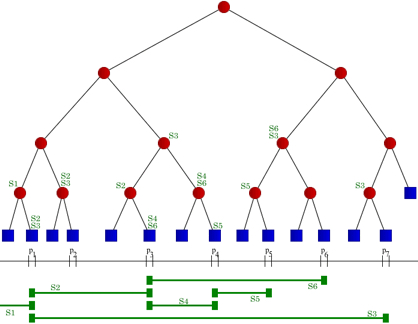
\includegraphics[scale=0.4]{segment_tree.jpg} 
\begin{description}
\item[Spatial complexity] $\bigoh(n\log(n))$
\item [Update time complexity] $\bigoh(\log(n))$
\item [Query time complexity] $\bigoh(\log(n))$
\item [Total Query time complexity] $\bigoh(m\log(n))$ $\Rightarrow$ \textit{\textbf{AC}}
\end{description}
\end{center}
\end{frame}
\subsection{Implementation}
\begin{frame}[fragile,allowframebreaks]
  \frametitle{Segment Tree implementation}
  \begin{lstlisting}
class SegmentTree {
  int[] st, A;
  int n;
  int left (int p) { return p << 1; }
  int right(int p) { return (p << 1) + 1; }

  void build(int p, int L, int R) {
    if (L == R)
      st[p] = L; // or R
    else {
      int mid = (L + R) / 2;
      build(left(p) , L      , mid);
      build(right(p), mid + 1, R);
      int p1 = st[left(p)], p2 = st[right(p)];
      st[p] = (A[p1] <= A[p2]) ? p1 : p2;
  } }

  int rmq(int p, int L, int R, int i, int j) { // O(log n)
    if (i >  R || j <  L) return -1;    // outside query  range
    if (i <= L && R <= j) return st[p]; // inside  query  range
    int mid = (L + R) / 2;
    int p1 = rmq(left(p) , L      , mid, i, j);
    int p2 = rmq(right(p), mid + 1, R  , i, j);

    if (p1 == -1) return p2;            // outside query  range
    if (p2 == -1) return p1;
    return (A[p1] <= A[p2]) ? p1 : p2; }

  int update(int p, int L, int R, int i, int j, int v) {
    if (i > R || j < L)                 // outside update range
      return st[p];
    //if (i <= L && R <= j) // could be lazy here !! Depends on application
    if (L == R) {
      A[i] = v;
      return st[p] = L; // or R
    }
    int mid = (L + R) / 2;
    int p1 = update(left(p) , L      , mid, i, j, v);
    int p2 = update(right(p), mid + 1, R  , i, j, v);
    return st[p] = (A[p1] <= A[p2]) ? p1 : p2;
  }

  public:

  SegmentTree(int[] _A) {
    A = _A; n = A.length;
    st = new int[4 * n];
    for (int i = 0; i < 4 * n; i++) st[i] = 0;
    build(1, 0, n - 1);
  }
  int rmq(int i, int j) { return rmq(1, 0, n - 1, i, j); }
  int update_point(int i, int v) {
    return update(1, 0, n - 1, i, i, v); }
  int update_interval(int i, int j, int v) {
    return update(1, 0, n-1, i, j, v); }
};
  \end{lstlisting}
  \begin{itemize}
    \item IOI-2013 day 2: ``game''
    \item \url{http://codeforces.com/problemset/problem/474/E}
  \end{itemize}
\end{frame}

\section{Fenwick Tree}
\begin{frame}[allowframebreaks,fragile]
  \frametitle{Fenwick Tree}
  Dynamic Range Sum Query

  What are the numbers smaller that $1011001000$ ?
  \begin{itemize}
    \item $1011000???$
    \item $1010??????$
    \item $100???????$
    \item $0?????????$
  \end{itemize}
  \begin{multline*}
    \mathsf{rsq}(1011001000)
    = \mathsf{ft}(1011001000)
    + \mathsf{ft}(1011000000)\\
    + \mathsf{ft}(1010000000)
    + \mathsf{ft}(1000000000)
  \end{multline*}

  \begin{lstlisting}
    adjust(01011001000,1):
        ft[01011010000]++
        ft[01011100000]++
        ft[01100000000]++
        ft[10000000000]++
  \end{lstlisting}

  \begin{lstlisting}
x             00000000000000000010010110100000
~x            11111111111111111101101001011111
-x or (~x)+1  11111111111111111101101001100000
x & (-x)      00000000000000000000000000100000
  \end{lstlisting}

  \framebreak
  \begin{lstlisting}
class FenwickTree {
  int *ft;
  int n;
  int LSOne(int S) { return (S & (-S)); }
  public:
  FenwickTree(int n) { // ignore index 0
    this->n = n;
    ft = new int[n+1];
    for (int i = 0; i <= n; i++) ft[n] = 0;
  }
  int rsq(int b) {        // returns RSQ(1, b)     PRE 1 <= b <= n
    int sum = 0; for (; b > 0; b -= LSOne(b)) sum += ft[b];
    return sum;
  }
  int rsq(int a, int b) { // returns RSQ(a, b)     PRE 1 <= a,b <= n
    return rsq(b) - (a == 1 ? 0 : rsq(a - 1));
  }
  void adjust(int k, int v) { // n = ft.size() - 1 PRE 1 <= k <= n
    for (; k <= n; k += LSOne(k)) ft[k] += v;
  }
};
  \end{lstlisting}
  \framebreak
  Exemples:
  \begin{itemize}
    \item NWERC 2011 Problem C
    \item \url{http://codeforces.com/contest/504/problem/B}
    \item \url{http://codeforces.com/problemset/problem/459/D}
  \end{itemize}
\end{frame}

\section{Sparse table}
\begin{frame}
  \frametitle{Sparse Table}
  Static Range Minimum Query

  $m[i][j]$ stores the smallest of $[i;i+2^j[$.

  $\min([a; b[) = \min(m[a][k], m[b-2^k][k])$ for $k$ such that
  $$2^{k-1} < b-a \leq 2^k$$
\end{frame}

\begin{frame}
  \frametitle{Tricky example}
  Get a tree flat with DFS then apply RSQ and RMQ.
  \begin{itemize}
    \item Least Common Ancestor: LCA
    \item \url{http://codeforces.com/contest/383/problem/C}
  \end{itemize}
\end{frame}

\end{document}
